\begin{blocksection}
\question Give the environment diagram and console output that result from running the following code.

\begin{lstlisting}
def swap(x, y):
    x, y = y, x
    return print("Swapped!", x, y)

x, y = 60, 1
a = swap(x, y)
swap(a, y)
\end{lstlisting}

\begin{solution}[2in]
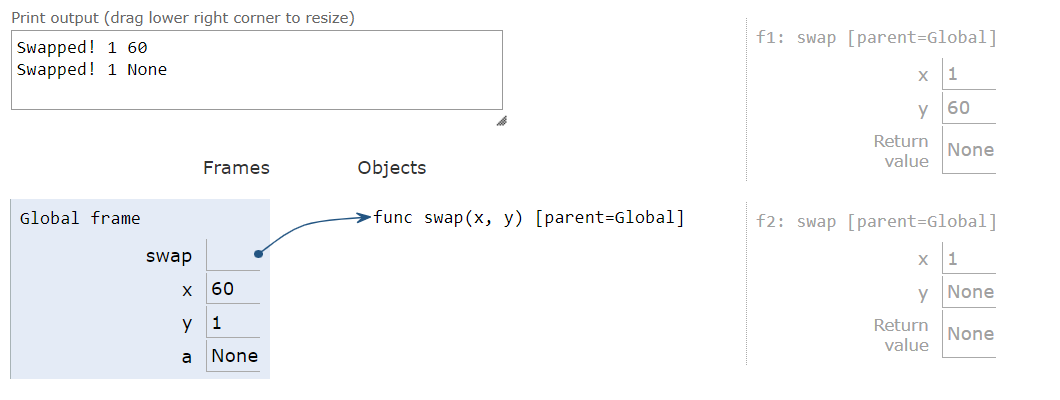
\includegraphics[scale=0.5]{swap.png}
\\
\url{https://tinyurl.com/y68m6qdj}
\end{solution}
\end{blocksection}

\begin{questionmeta}
\textbf{Teaching Tips}
  \begin{itemize}
    \item It's important to explain the difference between pass by reference and pass by value with x and y
    \item It is also important to explain the difference between printing and returning, which can be confusing to students at the beginning
  \end{itemize}
\end{questionmeta}
